% Source for the figure of PackedArray and TritArray (sec. 22.7): a word of
% PackedArray<4> with its 16 fields, the field 5 written by set(5, 9), and
% a byte of TritArray with its five digits in base 3, the digit 2 written by
% set(2, 0). Build: make figures (in ../build).
\documentclass[border=4pt]{standalone}
\usepackage[T1]{fontenc}
\usepackage{lmodern}
\usepackage{amsmath}
\usepackage{tikz}
\usepackage{lamalunga}
% tikz-ads.tex: the TikZ styles shared by the figures of the memory of the
% manual, \input by each standalone figure: a cell of a vector (cell), the
% cell that an operation touches (touched), a free cell (free), a node of a
% linked structure (node), the labels of indices (index) and of variables
% (var), a pointer (ptr), and \cells and \indices to draw a row of cells.
\usetikzlibrary{arrows.meta,positioning,calc,fit,shapes.multipart}
\definecolor{adsTouched}{RGB}{214,196,236}
\definecolor{adsFree}{RGB}{236,236,236}
\tikzset{
  ads/.style={>={Stealth[length=2mm]},font=\small,
              every node/.append style={inner sep=0pt}},
  cell/.style={draw,minimum width=7mm,minimum height=7mm,
               font=\small\ttfamily,outer sep=0pt},
  touched/.style={cell,fill=adsTouched},
  free/.style={cell,fill=adsFree,text=black!45},
  node/.style={draw,rounded corners=1pt,minimum width=8mm,
               minimum height=6mm,font=\small\ttfamily},
  index/.style={font=\scriptsize\ttfamily,text=black!60},
  var/.style={font=\small\itshape},
  ptr/.style={->,thick}
}
% \cells{name}{x,y}{list}: a row of cells, the first at (x,y), named
% name-0, name-1, ...; each item is text/style, the style one of cell,
% touched and free (e.g., {a/cell,e/touched,/free})
\newcommand{\cells}[3]{%
  \foreach \v/\s [count=\i from 0] in {#3}
    \node[\s] (#1-\i) at ($(#2)+(\i*7mm,0)$) {\v};}
% \indices{name}{n}: the indices 0 .. n-1 under the cells of name
\newcommand{\indices}[2]{%
  \foreach \i in {0,...,\numexpr#2-1\relax}
    \node[index,below=1.2mm of #1-\i] {\i};}

\begin{document}
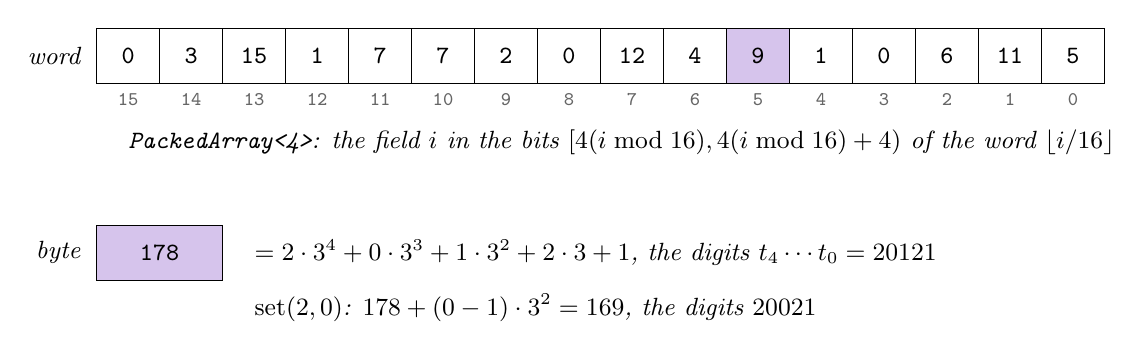
\begin{tikzpicture}[ads,f/.style={cell,minimum width=8mm}]
  \node[var,anchor=east] at (-6mm,0) {word};
  \foreach \v/\s [count=\k from 0] in {0/f,3/f,15/f,1/f,7/f,7/f,2/f,0/f,
      12/f,4/f,9/touched,1/f,0/f,6/f,11/f,5/f}
    \node[\s,minimum width=8mm] (p\k) at (\k*8mm,0) {\v};
  \foreach \k in {0,...,15}
    \node[index,below=1.2mm of p\k] {\pgfmathtruncatemacro\i{15-\k}\i};
  \node[var,anchor=west] at (0,-11mm)
    {\texttt{PackedArray<4>}: the field $i$ in the bits $[ 4 ( i \bmod 16 ) , 4 ( i \bmod 16 ) + 4 )$ of the word $\lfloor i / 16 \rfloor$};
  \node[var,anchor=east] at (-6mm,-25mm) {byte};
  \node[touched,minimum width=16mm] (y) at (4mm,-25mm) {178};
  \node[var,anchor=west] at (16mm,-25mm)
    {$= 2 \cdot 3^4 + 0 \cdot 3^3 + 1 \cdot 3^2 + 2 \cdot 3 + 1$, the digits $t_4 \cdots t_0 = 20121$};
  \node[var,anchor=west] at (16mm,-32mm)
    {$\mathrm{set}( 2 , 0 )$: $178 + ( 0 - 1 ) \cdot 3^2 = 169$, the digits $20021$};
\end{tikzpicture}
\end{document}
